\documentclass[nofooter,landscape,scale=1.4]{poster}
\usepackage[absolute,overlay]{textpos}

\usepackage{ragged2e}
\usepackage{pgfplots}
\usepackage[ruled]{algorithm}
\usepackage{algpseudocode}
\usepackage{nicefrac}




\newcommand{\ubar}[1]{\underline{#1\mkern-3mu}\mkern3mu }

\setlength{\TPHorizModule}{1cm}
\setlength{\TPVertModule}{1cm}

\title{Causal Bandits: Learning Good Interventions via Causal Inference}
\author{\mbox{}\\[1.3cm] Finnian Lattimore \hspace{2cm} Tor Lattimore \hspace{2cm} Mark Reid}
\footer{Contact}
\date{}

\begin{document}
\begin{frame}

%%%%%%%%%%%%%%%%%%%%%%%%%%%%%%%%%%%%%%%%%%%%%%%%%
% INTRODUCTION
%%%%%%%%%%%%%%%%%%%%%%%%%%%%%%%%%%%%%%%%%%%%%%%%%
\begin{textblock}{25.33}(2,12)
%\setbeamercolor*{block body}{bg=,fg=black}
\begin{block}{Introduction}
\justifying
We study the problem of using causal models to improve the rate at which good interventions can be learned online in a stochastic environment. 
Our formalism combines multi-arm bandits and causal inference to model a novel type of bandit feedback that is not exploited by existing approaches.
We propose a new algorithm that exploits the causal feedback and prove a bound on its simple regret that is strictly better (in all quantities) 
than algorithms that do not use the additional causal information.

\eq{
&\textbf{upper-bound, } R \in \bigo{\sqrt{\frac{m(\vec{q})}{T}\log\left(\frac{NT}{m(\vec{q})}\right)}}\,.\\
&\textbf{lower-bound, }R \in \Omega\left(\sqrt{\frac{m(\vec{q})}{T}}\right)\,.\\
&\textbf{standard lower-bound, }\simpleregret \in \Omega\left(\sqrt{\frac{N}{T}}\right)\,.
}
\end{block}

\begin{block}{Model}
\begin{itemize}
\item $K$ jobs 
\item Unknown parameters $\nu_1,\ldots,\nu_K$ with $\nu_k \geq 0$
\item At the start of each time step $t$ the learner chooses resource allocation $M_{k,t}$
\item Resources are limited: $\sum_{k=1}^K M_{k,t} \leq 1$
\item Job $k$ succeeds with probability $\min\set{1, M_{k,t} / \nu_k}$
\end{itemize}
\vspace{0.5cm}
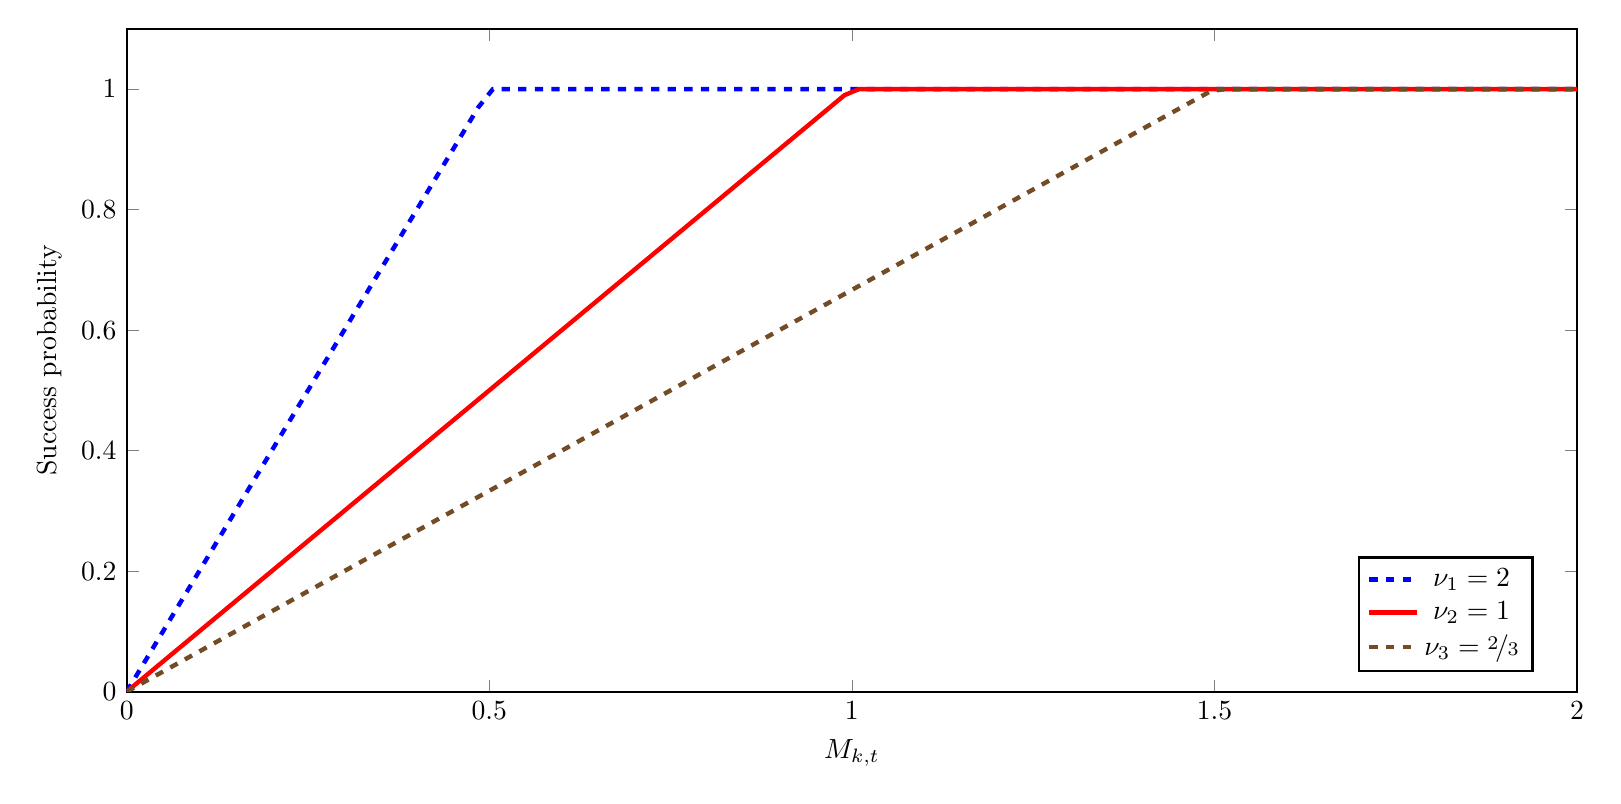
\begin{tikzpicture}[thick]
  \begin{axis}[thick,xlabel={$M_{k,t}$},ylabel={Success probability},width=20cm,height=10cm,scaled ticks=false,xmin=0,xmax=2,ymin=0,xtick={0,0.5,1,1.5,2},legend pos=south east] 
    \addplot+[dashed,mark=none,domain=0:2,samples=100,ultra thick] {and(\x<0.5,\x>=0)*2*\x + and(\x>=0.5,\x<=2)*1};
    \addlegendentry{$\nu_1 = 2$};
    \addplot+[mark=none,domain=0:2,samples=100,ultra thick] {and(\x<1,\x>=0)*\x + and(\x>=1,\x<=2)*1};
    \addlegendentry{$\nu_2 = 1$};
    \addplot+[dashed,mark=none,domain=0:2,samples=100,ultra thick] {and(\x<1.5,\x>=0)*\x*2/3 + and(\x>=1.5,\x<=2)*1};
    \addlegendentry{$\nu_3 = \nicefrac{2}{3}$};
  \end{axis}
\end{tikzpicture}
\begin{itemize}
\item All jobs are restarted after every time step
\item Goal is to maximise the expected number of successful jobs up to known time step $n$
\eq{
\sum_{t=1}^n \sum_{k=1}^K \min\set{1, {M_{k,t} \over \nu_k}}
}
\item $M^*_k$ is the unknown optimal allocation (computed by allocating resources to easiest jobs first)
\end{itemize}
\end{block}


\begin{block}{Regret}
\justifying
The expected regret $R_n$ of an algorithm measures the difference between the optimal allocation and the allocation of the algorithm
\eq{
\E\left[\sum_{t=1}^n \sum_{k=1}^K \left( \min\set{1, {M^*_k \over \nu_k}} - \min\set{1, {M_{k,t} \over \nu_k}}\right)\right]
}
An algorithm is learning if the expected regret is sub-linear: $\lim_{n\to\infty} R_n / n = 0$ \\[1cm]

Minimising the regret in this setting is especially challenging since
over-allocation resources to a job provides only limited information, while under-allocating risks severe sub-optimally.
\end{block}

\end{textblock}

\begin{textblock}{25.33}(29.33,12)
\begin{block}{Estimation}
\begin{itemize}
\item Algorithm works by estimating $\nu_k$ 
\item $X_{k,s} = \ind{\text{job } k \text{ completed in time step } s}$
\item If $M_{k,s} \leq \nu_k$, then ${1 \over \nu_k} = \E[X_{k,s} / M_{k,s}]$
\item Small/large $M_{k,s}$ implies large/small variance
\item Suggests a weighted estimator
\eq{
w_{k,t} &\leftarrow {1 \over 1 - {M_{k,t} \over \bar \nu_{k,t-1}}} 
&{1 \over \hat\nu_{k,t}} &\leftarrow {\sum_{s=1}^{t} w_{k,s} X_{k,s} \over \sum_{s=1}^t w_{k,s} M_{k,s}} 
}
\item $\bar \nu_{k,t-1}$ is a high-probability upper bound on $\nu_k$ obtained in previous time step
\item Confidence bounds about $\hat \nu_k$ are obtained via a modified version of Bernstein's inequality
\end{itemize}
\end{block}

\vspace{-1cm}
{
%\setbeamercolor*{block body}{bg=white!95!blue,fg=black}
\begin{block}{Optimistic Algorithm}
\begin{algorithmic}[1]
\State {\bf input: } $n, K$, $\set{\ubar \nu_{k,0}}_{k=1}^K$
\State $\delta \leftarrow (nK)^{-2}$ and $\bar \nu_{k,0} = \infty$ for each $k$
\For{$t \in 1, \ldots, n$}
\State /* Optimistically choose $M_{k,t}$ using $\ubar \nu_{k,t-1}$ */
\State $(\forall k \in 1,\ldots,K)$ initialise $M_{k,t} \leftarrow 0$
\For{$i \in 1, \ldots, K$}
\State $k \leftarrow \argmin\limits_{k : M_{k,t} = 0} \ubar \nu_{k,t-1}$
\State $M_{k,t} \leftarrow \min \set{\ubar \nu_{k,t-1},\; 1 - \sum_{j=1}^K M_{j,t}}$
\EndFor
\State $(\forall k \in 1,\ldots,K)$ observe $X_{k,t}$ 
\State $(\forall k \in 1,\ldots,K)$ compute estimates:
\eq{
w_{k,t} &\leftarrow {1 \over 1 - {M_{k,t} \over \bar \nu_{k,t-1}}} 
&{1 \over \hat\nu_{k,t}} &\leftarrow {\sum_{s=1}^{t} w_{k,s} X_{k,s} \over \sum_{s=1}^t w_{k,s} M_{k,s}} 
}
\State $(\forall k \in 1,\ldots,K)$ update confidence intervals:
\eq{
R_{k,t} &\leftarrow \max_{s \leq t} w_{k,s}  \qquad \hat V^2_{k,t} \leftarrow \sum_{s \leq t} {w_{k,s} M_{k,s} \over \ubar \nu_{k,t-1}} \\
\tilde \epsilon_{k,t} &\leftarrow {f(R_{k,t}, \hat V^2_{k,t},\delta) \over \sum_{s=1}^t w_{k,s} M_{k,s}}    \\
{1 \over \ubar \nu_{k,t}} &\leftarrow \min\set{{1 \over \ubar \nu_{k,t-1}}, {1 \over \hat \nu_{k,t}} + \tilde\epsilon_{k,t}} \\
{1 \over \bar \nu_{k,t}} &\leftarrow \max\set{{1 \over \bar \nu_{k,t-1}}, {1 \over \hat \nu_{k,t}} - \tilde\epsilon_{k,t}} 
}
\EndFor
\Statex 
\Function{$f$}{$R$,$V^2$, $\delta$}
\State $\delta_0 \leftarrow {\delta \over 3(R+1)^2 (V^2+1)^2}$
\State \Return 
${R+1 \over 3} \log{2 \over \delta_0}$
\Statex $\qquad +\;\;\sqrt{2(V^2+1) \log{2 \over \delta_0} + \left({R+1 \over 3}\right)^2 \log^2{2 \over \delta_0}}$
\EndFunction
\end{algorithmic}
\end{block}
}

\vspace{-1cm}
\begin{block}{Bounds on the Regret}
\vspace{-2.5cm}
\eq{
&R_n \in O\Bigg(\ell \log^2 n + \sum_{k=\ell+1}^K \left(\log {1 \over \nu_k \Delta_{\ell,k}}\right)\log n  \\
\nonumber &\;\;+\sum_{k=\ell+2}^K \left(\log{1 \over \nu_k \Delta_{\ell+1,k}}\right) \log n
+ \sum_{k=\ell+1}^K {\log n \over \Delta_{\ell+1,k}} \Bigg),
}
\begin{itemize}
\item $\ell$ is the number of jobs that are fully allocated under the optimal allocation and $\Delta_{i,j} = {1 \over \nu_{i}} - {1 \over \nu_j}$
\item If all jobs can be fully allocated, then bound is independent of the gaps
\item $\Omega(\sqrt{K n})$ problem-independent lower bound
\end{itemize}

\end{block}

\end{textblock}

\begin{textblock}{25.33}(56.66,12)
\begin{block}{Experiments}
\begin{itemize}
\item Code and data available in supplementary material
\item Data points based on mean of 300 samples
\end{itemize}

\vspace{0.5cm}
\begin{minipage}{17cm}
\begin{tikzpicture}[baseline,font=\scriptsize]
  \begin{axis}[xlabel shift=-5pt,xmax=10,ylabel shift=-5pt,xlabel={$\nu_2$},ylabel={$R_n$},xmin=2,ymin=110,height=10cm,width=15cm,mark size=2pt,compat=newest,xtick={2,3,4,5,6,7,8,9,10}]
    \addplot+[only marks] table {exp1.txt};
  \end{axis}
\end{tikzpicture}
\end{minipage}
\begin{minipage}{6cm}
$K = 2$ \\
$n = 10^4$ \\ 
$\nu_1 = 2$ \\ 
$\nu_2 \in [2,10]$
\end{minipage}

\hspace{-1cm}
\begin{minipage}{17cm}
\begin{tikzpicture}[baseline,font=\scriptsize]
  \begin{axis}[xlabel shift=-5pt,ylabel shift=-5pt,xlabel={$n$},ylabel={$\displaystyle {R_n \over \log^2 n}$},compat=newest,mark size=2pt,height=10cm,scaled ticks=false,width=15cm,xtick={0,1000000},xticklabels={0,1e6}] 
    \addplot+[only marks] table {exp2.txt};
  \end{axis}
\end{tikzpicture}
\end{minipage}
\hspace{0.3cm}
\begin{minipage}{6cm}
$K = 2$ \\
$\nu_1 = \nicefrac{4}{10}$ \\
$\nu_2 = \nicefrac{6}{10}$
\end{minipage}

\begin{minipage}{17cm}
\begin{tikzpicture}[font=\scriptsize]
  \begin{axis}[xtick={0.35,0.60,1.05},ytick={2000,5000},yticklabels={2e3,5e3},xlabel shift=-5pt,ylabel shift=-5pt,xlabel={$\nu_2$},ylabel={$R_n$},compat=newest,mark size=2pt,height=10cm,width=15cm] 
    \addplot+[only marks] table {exp3.txt};
  \end{axis}
\end{tikzpicture}
\end{minipage}
\begin{minipage}{6cm}
$K = 2$ \\
$n = 10^5$ \\ 
$\nu_1 = \nicefrac{4}{10}$ \\
$\nu_2 \in [\nicefrac{4}{10},1]$
\end{minipage}

\begin{minipage}{17cm}
\begin{tikzpicture}[font=\scriptsize]
  \begin{axis}[ytick={0,10000},yticklabels={0,1e4},xlabel shift=-5pt,ylabel shift=-5pt,scaled ticks=false,xlabel={$n$},ylabel={$R_n$},compat=newest,mark size=2pt,height=10cm,width=15cm,xtick={0,100000},xticklabels={0,1e5}] 
    \addplot+[only marks,blue] table[x index=0,y index=1] {exp4.txt};
    \addplot+[each nth point=3, filter discard warning=false, unbounded coords=discard,only marks,red] table[x index=0,y index=2] {exp4.txt};
  \end{axis}
\end{tikzpicture}
\end{minipage}
\begin{minipage}{6cm}
$K = 2$ \\
$\nu_1 = \nicefrac{4}{10}$ \\
$\nu_2 = \nicefrac{6}{10}$ \\
\tikz[baseline=-0.5ex]{\draw[line width=0.1cm,blue] (0,0) -- (1,0);} {\small weighted} \\
\tikz[baseline=-0.5ex]{\draw[line width=0.1cm,red] (0,0) -- (1,0);} {\small unweighted} \\
\end{minipage}

\end{block}

\begin{block}{Applications}
\begin{itemize}
\item Cache allocation
\item Load balancing
\item Resource allocation is a common problem
\end{itemize}
\end{block}

\begin{block}{Summary}
\begin{itemize}
\item Introduced resource allocation setting
\item New algorithm is both practical and computationally efficient
\item Nearly-optimal adaptive bounds on the regret
\item Weighted estimators independently interesting
\end{itemize}
\end{block}

\begin{block}{Open Questions}
\begin{itemize}
\item Reduce $\log^2 n$ dependence to $\log n$
\item Algorithm is not anytime
\item Problem-dependent lower bounds
\item Non-parametric models (such as concave, piecewise linear, or monotonic)
\item Adversarial models
\item Variable rewards for each job
\item Resources not replenished each time step
\item Many more!
\end{itemize}
\end{block}

\end{textblock}




\end{frame}



\end{document}
